\documentclass[10pt, t, xcolor={usenames,dvipsnames,svgnames}, compress]{beamer}

\usepackage{booktabs}
\usepackage{dcolumn}
\usepackage{colortbl}
\usepackage{ifxetex}
\usepackage{amsmath}
\usepackage[style=authoryear-comp]{biblatex}
\usepackage[no-math]{fontspec}

\definecolor{untractable_red}{RGB}{209, 25, 25}
\definecolor{tractable_green}{RGB}{0, 153, 51}

\usetheme{enziteto}

\setbeamertemplate{headline}{}

\newcommand{\argmax}{\operatornamewithlimits{argmax}}

\addbibresource{../referomnia/referomnia.bib}

\title{Learning Sum-Product Networks}
\author{Nicola Di Mauro \and Antonio Vergari}
\date{September 2016}
\institute{Università degli Studi di Bari}
\department{Dipartimento di Informatica}
\laboratory{LACAM}
\group{Machine Learning}
\institutelogo{
\includegraphics[width=25pt]{figures/unibaba}}
\lablogo{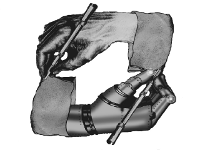
\includegraphics[width=35pt]{figures/lacam}}

%\footnotesize \let\small\footnotesize

\setbeamerfont{footnote}{size=\scriptsize}
\addtobeamertemplate{footnote}{}{\vspace{16pt}}

\begin{document}

\begin{frame}[c]
  \setbeamertemplate{headline}{}
  \setbeamertemplate{footline}{}
  \titlepage
\end{frame}

\begin{frame}
\frametitle{The need for SPN}
Sum-Product Networks (SPNs) are a type of probabilistic model\footnote{H. Poon
  and P. Domingos, \emph{Sum-Product Network: a New Deep Architecture}, UAI 2011}
\begin{itemize}
\item for Pobabilistic Graphical Models (PGMs) there exist multi-purpose
  inference tools
\begin{itemize}
\item the computational
effort scales unproportional to the complexity of the graph
\item solution: using approximate inference
\end{itemize}
\end{itemize}
\end{frame}

\begin{frame}[t]
  \frametitle{The need for SPNs}
  \framesubtitle{Why should you work on SPNs?}
\begin{itemize}
\item exact tractable inference
  \item NN for which structure learning is easy
\end{itemize}
SPNs represent probability distributions and a corresponding exact inference
machine for the represented distribution at the same time 
\end{frame}

\section{Representation}
{\setbeamertemplate{headline}{}
  \begin{frame}[c]
    \sectionpage
  \end{frame}
}

\begin{frame}
  \frametitle{Density estimation}
\end{frame}

\begin{frame}
  \frametitle{(Different kinds of) Inference}
  Different kinds of queries:
  \begin{itemize}
  \item $p(\mathbf{X})$ (evidence)
  \item $p(\mathbf{E}), \mathbf{E}\subset\mathbf{X}$ (marginals)
  \item $p(\mathbf{Q}|\mathbf{E}), \mathbf{Q},
    \mathbf{E}\subset\mathbf{X}, \mathbf{Q}\cap \mathbf{E}=\emptyset$ (conditionals)
  \item
    $\arg\max_{\mathbf{q}\sim\mathbf{Q}}p(\mathbf{q}|\mathbf{E})$
    (MPE assignment)
    \item complex queries
  \end{itemize}
\end{frame}

\begin{frame}
  \frametitle{Tractable Probabilistic Models}
\end{frame}

\begin{frame}
  \frametitle{Sum-Product Networks}
\end{frame}

\begin{frame}
  \frametitle{Scopes}
\end{frame}

\begin{frame}
  \frametitle{Structural Properties}
\end{frame}

\section{Inference}
{\setbeamertemplate{headline}{}
  \begin{frame}[c]
    \sectionpage
  \end{frame}
}

\begin{frame}
  \frametitle{Complete evidence}
\end{frame}

\begin{frame}
  \frametitle{Marginal inference}
\end{frame}

\begin{frame}
  \frametitle{MPE inference}
\end{frame}


\section{Interpretation}
{\setbeamertemplate{headline}{}
  \begin{frame}[c]
    \sectionpage
  \end{frame}
}

\begin{frame}
\frametitle{Interpretation}
\begin{itemize}
\item probabilistic model
\item deep feedforward neural network
\end{itemize}
\end{frame}


\begin{frame}
\frametitle{Network Polynomials}
\end{frame}

\begin{frame}
  \frametitle{Arithmetic Circuits}
  Differences with ACs:
  \begin{itemize}
  \item probabilistic semantics
    \begin{itemize}
    \item learning
      \item sampling
    \end{itemize}
    \item no shared weights
  \end{itemize}
\end{frame}

\begin{frame}[t]
  \frametitle{SPNs as NNs (I)}
  SPNs are a particular kind of \emph{\textbf{labelled}
    \textbf{constrained} and \textbf{fully probabilistic}}
  neural networks.\par\bigskip
  
  \textbf{Labelled}: each neuron is associated a \emph{scope}\par
  \textbf{Constrained}: completeness and decomposability determine
  network topology.\par
  \textbf{Fully probabilistic:} each valid sub-SPN is still a
  valid-SPN.\footfullcitenomarkleft{Vergari2016a}\par\bigskip
  
  SPNs provide a direct encoding of the input space into a deep
  architecture $\rightarrow$ \emph{\textbf{visualizing representations}} (back) into the \emph{\textbf{input space}}.
\end{frame}

\begin{frame}
  \frametitle{SPNs as NNs (II)}
  \small
  A classic MLP hidden layer computes the function:
  $$h(\mathbf{x}) =\sigma(\mathbf{W}\mathbf{x}+ \mathbf{b})$$

  SPNs can be reframed as \textit{DAGs} of MLPs, each sum layer
  computing:
  $$\mathbf{S}(\mathbf{x}) =
  \log(\mathbf{W}\mathbf{x})$$
  and product layers computing:
  $$\mathbf{S}(\mathbf{x}) = \exp(\mathbf{P}\mathbf{x})$$
  where
  $\mathbf{W}\in\mathbb{R}_{+}^{s\times r}$ and $\mathbf{P}\in\{0,
  1\}^{s\times r}$ are the weight matrices:
  \begin{equation*}
    \mathbf{W}_{(ij)}= \begin{cases}
      w_{ij} &\text{if $i\rightarrow j$}\\
      0& \text{otherwise}
    \end{cases}\quad\quad\mathbf{P}_{(ij)}=
    \begin{cases}
      1 &\text{if $i\rightarrow j$}\\
      0& \text{otherwise}
    \end{cases}
  \end{equation*}\footfullcitenomarkleft{Vergari2016a}
\end{frame}

\begin{frame}
  \frametitle{SPNs as NNs (III)}
  \begin{center}
    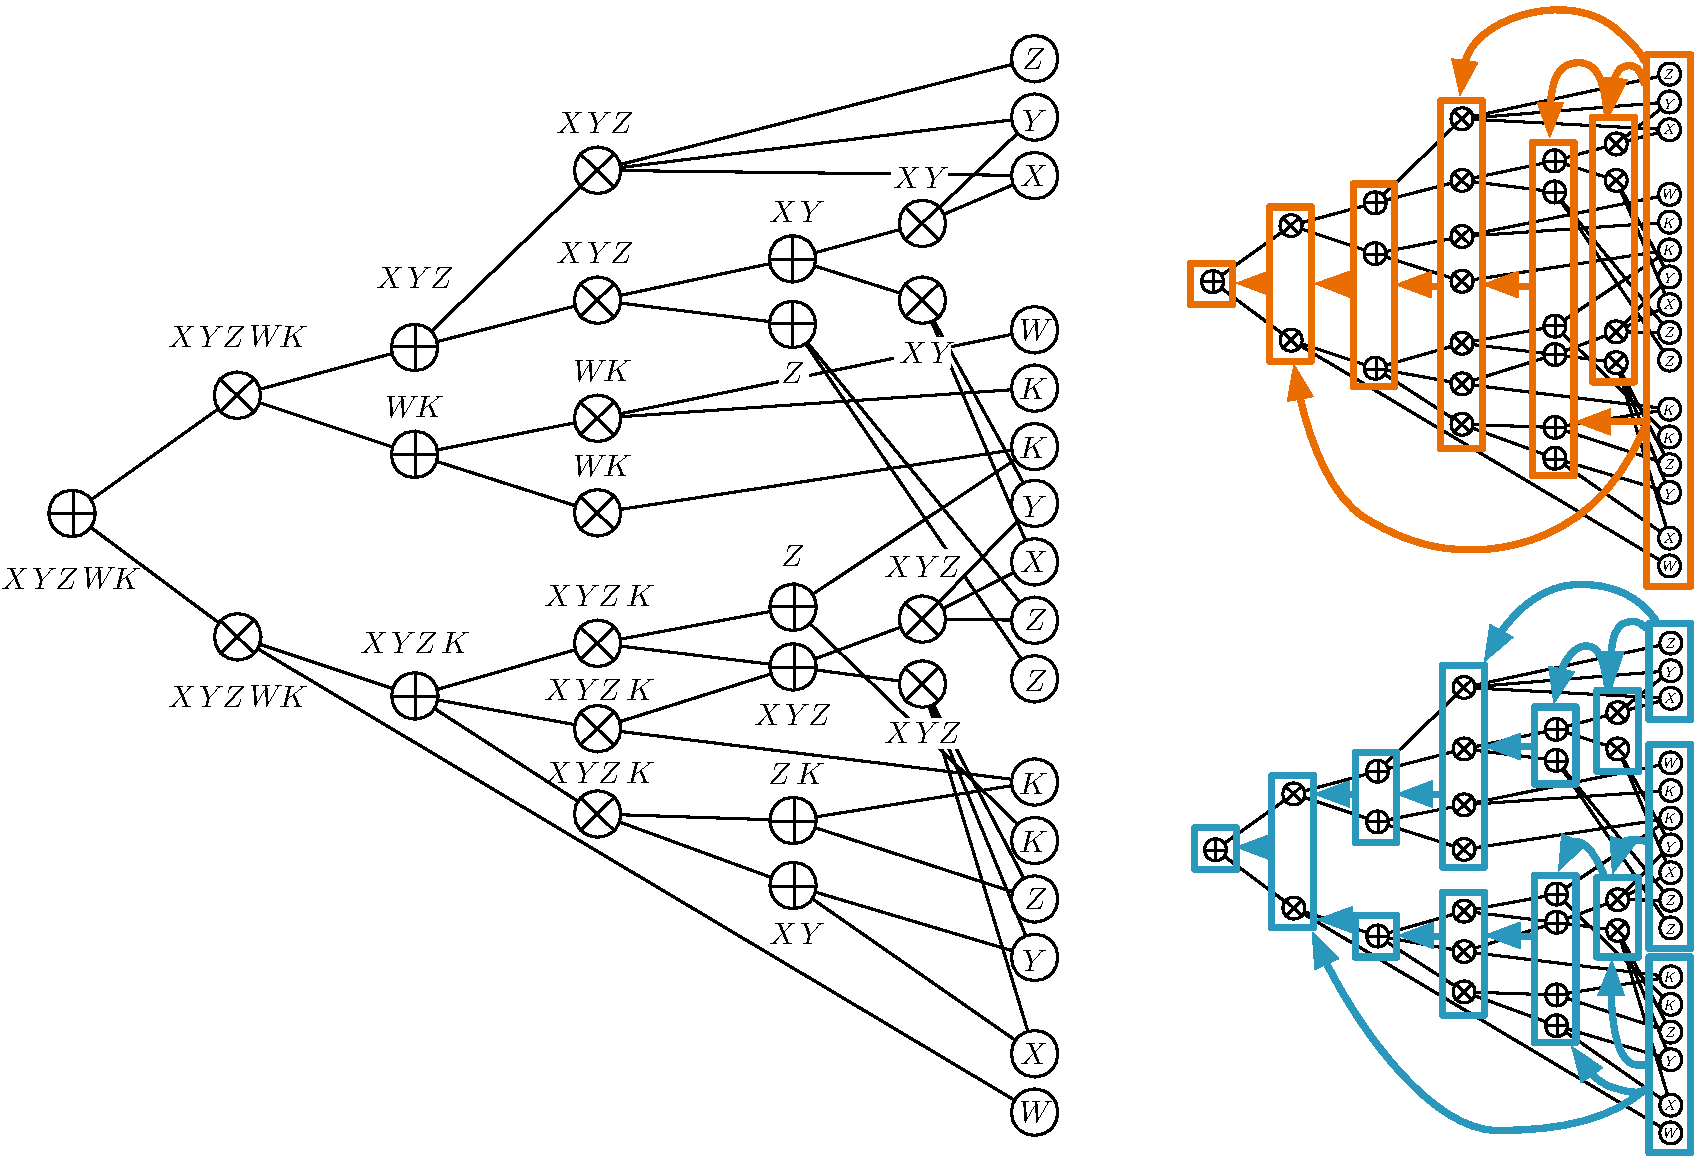
\includegraphics[width=0.8\columnwidth]{figures/layered-spn.pdf}
  \end{center}
\end{frame}

\begin{frame}
  \frametitle{SPNs as NNs (IV): filters}
  \small
  Learned features as images maximizing neuron activations~\parencite{Erhan2009}:
  $$\mathbf{x}^{*} = \argmax_{\mathbf{x},
    ||\mathbf{x}||=\gamma}h_{ij}(\mathbf{x};\boldsymbol\theta).$$
  With SPNs, joint solution as an MPE assignment for all nodes (linear time):
  $$\mathbf{x}^{*}_{|\mathsf{sc}(n)} =
  \argmax_{\mathbf{x}}S_{n}(\mathbf{x}_{|\mathsf{sc}(n)};
  \mathbf{w})$$.
  \begin{center}
    \vspace{-15pt}
    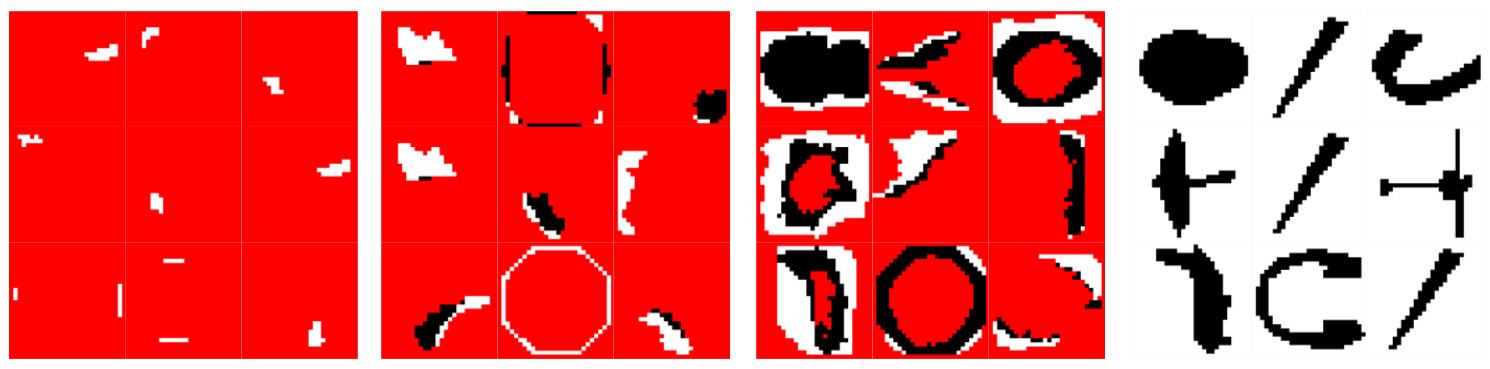
\includegraphics[width=0.9\linewidth]{figures/filters.jpg}
  \end{center}
  \footfullcitenomarkleft{Vergari2016a}
  $\rightarrow$ \emph{scope length} ($|\mathsf{sc}(n)|$) correlates with feature abstraction level
\end{frame}

\begin{frame}
  \frametitle{SPNs as BNs I}
  Zhao and Poupart
\end{frame}

\begin{frame}
  \frametitle{SPNs as BNs II}
  Peharz
\end{frame}

\begin{frame}
  \frametitle{Myths about SPNs}
 \textbf{SPNs are PGMs}. false

 \textbf{SPNs are convolutional NNs}. false

  SPNs 
\end{frame}

\section{Learning}
{\setbeamertemplate{headline}{}
  \begin{frame}[c]
    \sectionpage
  \end{frame}
}

\begin{frame}
  \small
  \frametitle{Structure Learning}
  Structure matters

  Alternatives:
  \begin{itemize}
  \item handcrafted structure, then weight learning~\parencite{Poon2011}
  \item random structures, then weight learning~\parencite{Rashwan2016}
    \item learned from data
  \end{itemize}
\end{frame}

\begin{frame}
  \frametitle{Why Structure Quality Matters}

  \footnotesize
  
  Tractable inference is guaranteed \emph{if the network size is polynomial} in \#
  vars.\par\bigskip

  Smaller networks, faster inference (comparing network sizes is better than comparing inference times).\par\bigskip

  \emph{Deeper} networks are possibly \emph{more expressively efficient}~\emph{\parencite{Martens2014,Zhao2015}}.\par\bigskip

  Structural simplicity as a bias: overcomplex networks may not generalize well.\par\bigskip
  
  Structure quality desiderata: \textbf{\textbf{smaller}} but \textbf{\textbf{accurate}}, \textbf{\emph{deeper}} but not
  wider, SPNs.
\end{frame}

\begin{frame}[t]
  \frametitle{LearnSPN (I)}
  \footnotesize
  Build a tree-like SPN by recursively split the data matrix:

  \begin{itemize}
  \item splitting columns into pairs by a greedy \textbf{\emph{G Test}} based
    procedure with threshold $\rho$:
    \[
      G(X_i, X_j) =  2\sum_{x_i \sim X_i}\sum_{x_j \sim X_j}c(x_i, x_j)\cdot \log\frac{c(x_i, x_j)\cdot |T|}{c(x_i)c(x_j)}
    \]
  \item clustering instances into $|C|$ sets with \textbf{\emph{online Hard-EM}} with cluster penalty
    $\lambda$:
    \[\begin{array}{cc}
        Pr(\mathbf{X})= \sum_{C_i \in \mathbf{C}}\prod_{X_j \in \mathbf{X}}Pr(X_j|C_i)Pr(C_i)\\
        % & Pr(C_i) \propto e^{-\lambda |\mathbf{C}|\cdot |\mathbf{X}|}\\
      \end{array}\]
    weights are estimated as cluster proportions
  \item if there are less than $m$ instances, put a \textbf{\emph{naive
        factorization}} over leaves
  \item each univariate distribution get \emph{\textbf{ML estimation}} smoothed by $\alpha$  
  \end{itemize}\par\bigskip

  Hyperparameter space: $\{\rho, \lambda, m, \alpha\}$.
  

\end{frame}

\begin{frame}
  \frametitle{LearnSPN (II)}
  \footnotesize
  \onslide<1-4>{\begin{minipage}[t]{0.3\linewidth}
      \begin{center}
        \only<1>{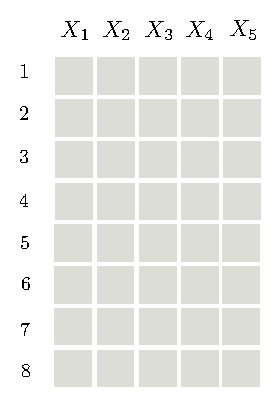
\includegraphics[width=0.8\linewidth]{figures/grid-0}}
        \only<2-4>{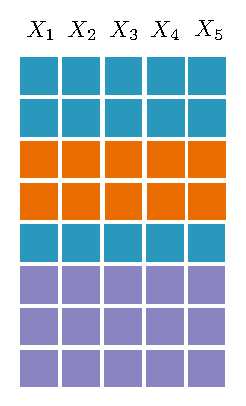
\includegraphics[width=0.715\linewidth]{figures/grid-1}}
      \end{center}
    \end{minipage}}\hspace{10pt}\onslide<3-4>{\begin{minipage}[t]{0.3\linewidth}
      \begin{center}
        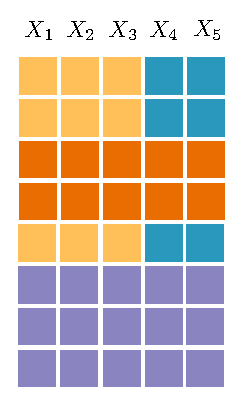
\includegraphics[width=0.72\linewidth]{figures/grid-2}
      \end{center}
    \end{minipage}}\hspace{10pt}\onslide<4>{\begin{minipage}[t]{0.3\linewidth}
      \begin{center}
        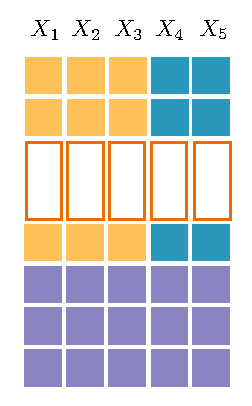
\includegraphics[width=0.735\linewidth]{figures/grid-3}
      \end{center}
    \end{minipage}}\\
  \vspace{15pt}
  \onslide<2-4>{\raisebox{0pt}{\begin{minipage}[t]{0.3\linewidth}
        \begin{center}
          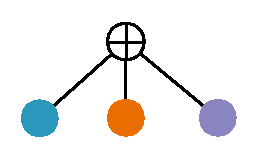
\includegraphics[width=0.715\linewidth]{figures/learnspn-1}
        \end{center}
      \end{minipage}}}\hspace{5pt}\onslide<3-4>{\raisebox{-25pt}{\begin{minipage}[t]{0.3\linewidth}
        \begin{center}
          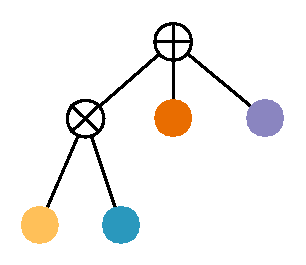
\includegraphics[width=0.83\linewidth]{figures/learnspn-2}
        \end{center}
      \end{minipage}}}\hspace{4pt}\onslide<4>{\raisebox{-22pt}{\begin{minipage}[t]{0.3\linewidth}
        \begin{center}
          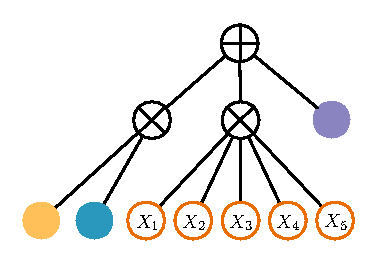
\includegraphics[width=1.0\linewidth]{figures/learnspn-3}
        \end{center}
      \end{minipage}}}
\end{frame}

\begin{frame}
  \frametitle{LearnSPN (III)}
  \footnotesize
  
  \textsf{LearSPN} performs two interleaved \textbf{\emph{greedy
      hierarchical}} divisive \textbf{\emph{clustering}}
  processes (co-clutering on the data matrix).\par\bigskip

  Fast and simple. But both processes never look back and are
  committed to the choices they take.\par\bigskip

  Online EM does not need to specify the number of clusters $k$ in
  advance. But overcomplex structures are learned by exploding the number of sum
  node children.\par\bigskip

  Tractable leaf estimation. But naive factorization independence
  assumptions may be too strong.\par\bigskip

  ML estimations are effective. But they are not robust to noise, they can overfit the training set easily.
\end{frame}

\begin{frame}
  \frametitle{LearnSPN}
\end{frame}

\begin{frame}
  \frametitle{LearnSPN-b}
  Observation: each clustering process benefits from the other one improvements/highly suffers
  from other's mistakes.\par\bigskip

  Idea: slowing down the processes by limiting the number of
  nodes to split into. \textsf{SPN-B}, variant of \textsf{LearnSPN} that uses EM
  for mixture modeling with
  $k=2$ to cluster rows.

  No need for $\lambda$ anymore.\par\bigskip

  \raisebox{45pt}{\begin{minipage}[t]{0.65\linewidth}
      Objectives:
      \begin{itemize}
      \item not committing to complex structures too early
      \item same expressive power as LearnSPN
      \item reducing node out fan increases the depth
      \item same accuracy, smaller networks
      \end{itemize}
    \end{minipage}}\hspace{-5pt}\begin{minipage}[t]{0.3\linewidth}
    \begin{center}
      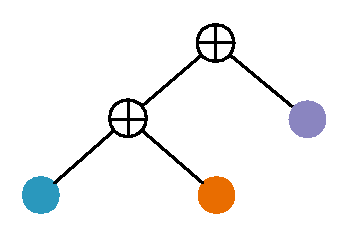
\includegraphics[width=0.9\linewidth]{figures/learnspn-4.pdf}
    \end{center}
  \end{minipage}
\end{frame}

\begin{frame}
  \frametitle{LearnSPN-b: depth VS size}

  \begin{figure}[htbp]
    \begin{center}
      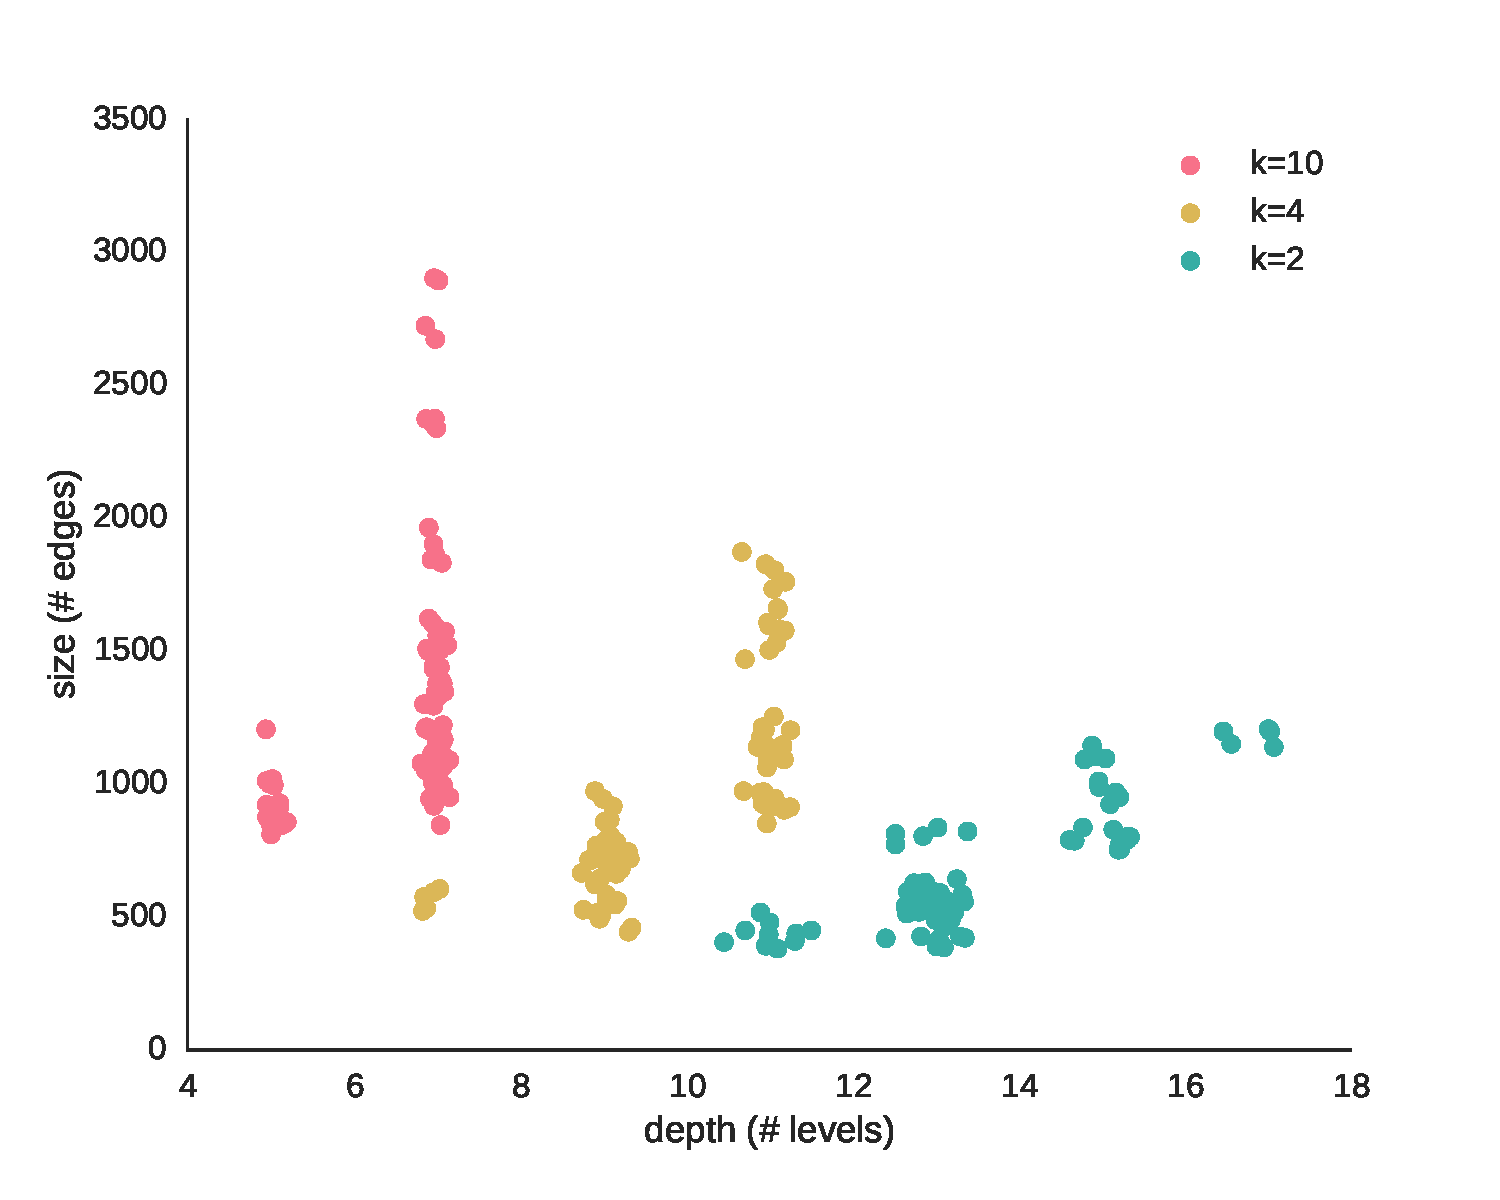
\includegraphics[width=0.5\linewidth]{figures/nltcs-depth.pdf}
      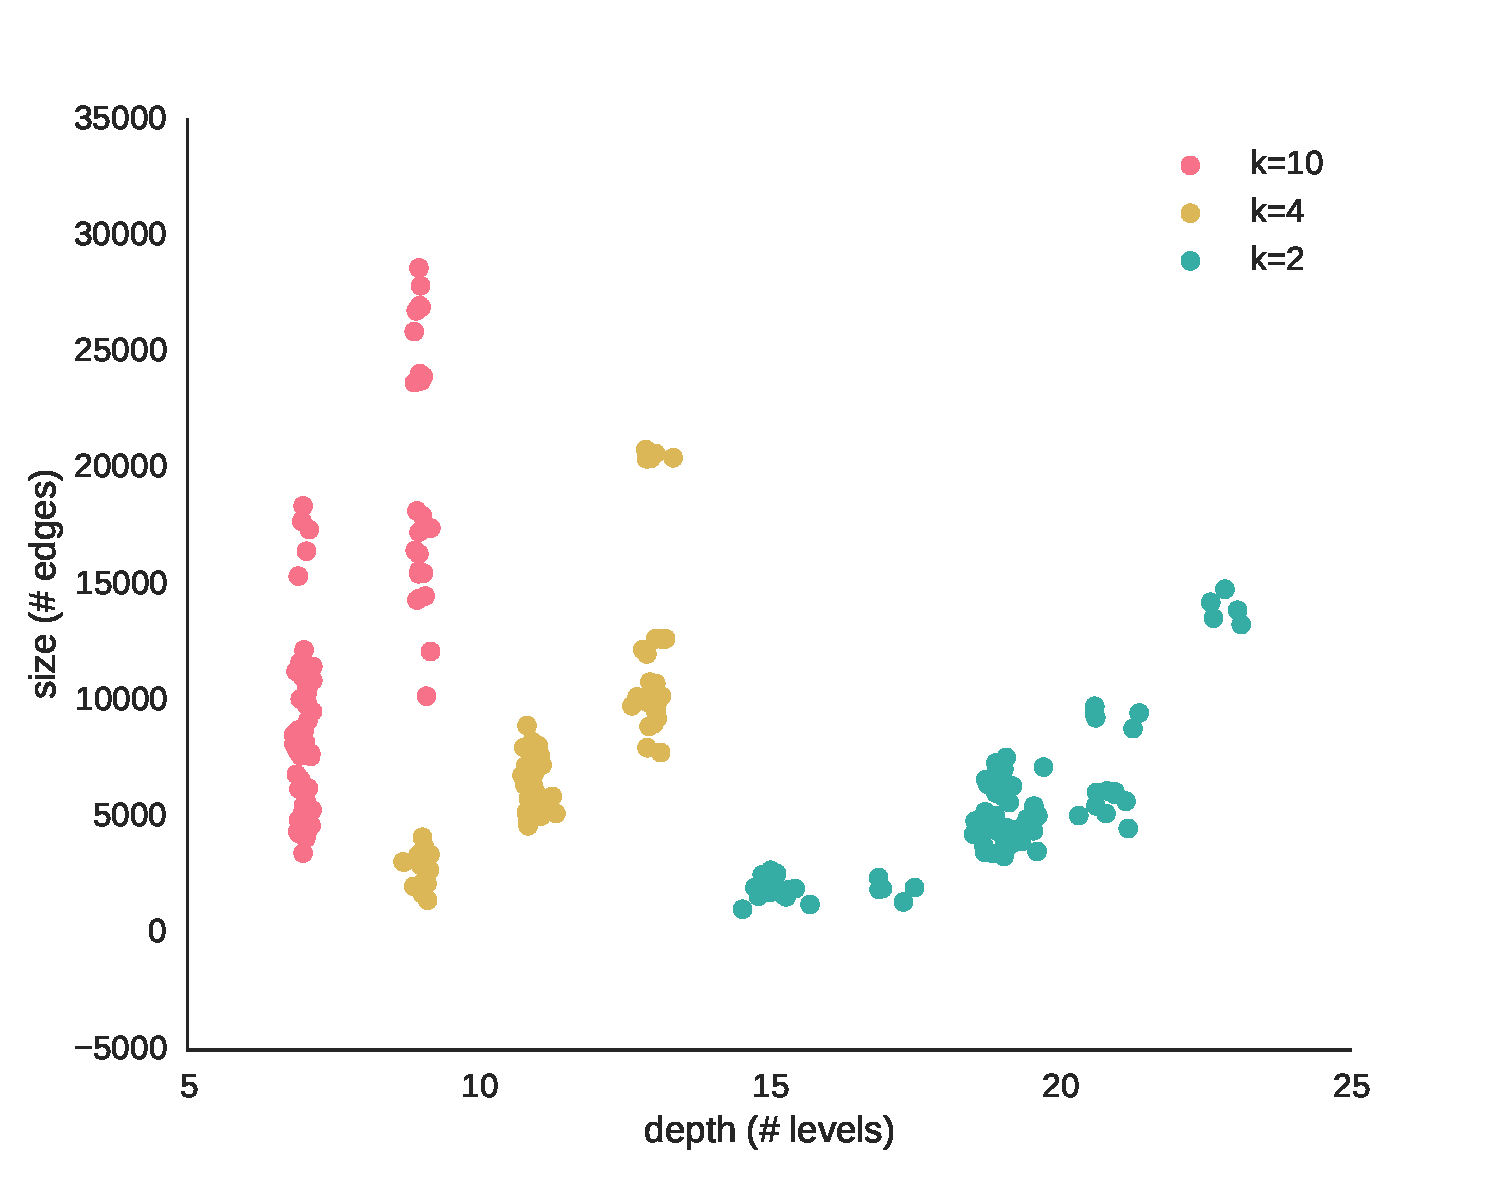
\includegraphics[width=0.5\linewidth]{figures/plants-depth.pdf}
      \caption{Comparing network sizes and depths while varying the max
        number of sum node children splits ($k\in\{10, 4, 2\}$). Each dot is an experiment
        in the grid search hyperparameter space performed by
        \textsf{SPN-B} on NLTCS (left) and Plants (right).}
    \end{center}
  \end{figure}

\end{frame}

\begin{frame}
  \frametitle{New Tendencies in Structure Learning}
  Pruning and compressing
\end{frame}

\begin{frame}
  \frametitle{Parameter Learning}
  Non convex optimization, solvable with iterative methods like: GD,
  EM,\dots\par\bigskip

  Use backpropagation ($\rightarrow$ differential approach) to compute
  $\nabla_{\mathbf{w}} S(\mathbf{x})$\par\bigskip

  Hard/Soft gradients\par\bigskip

  Some issues:
  \begin{itemize}
  \item vanishing gradients
    \item hyperparameter choices
  \end{itemize}
\end{frame}

\begin{frame}
  \frametitle{Hard/Soft Parameter Learning}
  \begin{table}
    \centering
    \begin{tabular}{l c c}
      &\textbf{soft}& \textbf{hard}\\
      \textsf{Generative Gradient} &$\frac{\partial
                                     S(\mathbf{x})}{\partial w_{pc}} =
                                     S_{c}(\mathbf{x})\frac{\partial
                                     S(\mathbf{x})}{\partial S_{p}(\mathbf{x})}$
                    &
                      $\frac{\sharp\{w_{pc}\in
                      \mathsf{MPE-path}(\mathbf{x})\}}{w_{pc}}$\\
      \textsf{Discriminative Gradient} & $\frac{1}{S(\mathbf{y}|\mathbf{x})}\frac{\partial
                                         S(\mathbf{y}|\mathbf{x})}{\partial
                                         w_{pc}} - \frac{1}{S(\mathbf{*}|\mathbf{x})}\frac{\partial
                                         S(\mathbf{*}|\mathbf{x})}{\partial
                                         w_{pc}}$ &
                                                    $\frac{\sharp\{w_{pc}\in
                                                    \mathsf{MPE-path}(\mathbf{y}|\mathbf{x})\}
                                                    - \sharp\sharp\{w_{pc}\in
                                                    \mathsf{MPE-path}(\mathbf{1}|\mathbf{x})\}}{w_{pc}}$\\
      \textsf{Generative Posterior} & $p(H_{p}=c|\mathbf{x})\propto \frac{1}{S(\mathbf{x})}\frac{\partial
                                      S(\mathbf{x})}{\partial S_{p}(\mathbf{x})}S_{c}(\mathbf{x})w_{pc}$ & $p(H_{p}=c|\mathbf{x})=
                                                                                             \begin{cases}
                                                                                               1
                                                                                               \text{if}
                                                                                               w
                                                                                               \in W
                                                                                               \\
                                                                                               0 \text{otherwise}
                                                                                             \end{cases}
$\\
    \end{tabular}
  \end{table}
\end{frame}

\begin{frame}
  \frametitle{Bayesian Parameter Learning}
\end{frame}

\begin{frame}[t]
  \frametitle{Parameter Learning VS LearnSPN}
  \begin{table}
    \centering
    \scriptsize
    \setlength{\tabcolsep}{3pt}  
    \begin{tabular}{l r r r r r r r}
      \toprule
      & \textsf{LearnSPN}\footcite{Gens2013} & \textsf{LearnSPN-b}\footcite{Vergari2015} & \textsf{CVB-SPN}\footcite{Zhao2016a} & \textsf{OBMM}\footcite{Rashwan2016} & \textsf{SGD}\footcite{Rashwan2016} & \textsf{EM}\footcite{Rashwan2016} & \textsf{SEG}\footcite{Rashwan2016} \\
      \midrule
      \textbf{NLTCS} & -6.11 & -6.05 & -6.08 & -6.07 & -8.76 & -6.31 & -6.85\\
      \textbf{MSNBC} & -6.11& -6.04& -6.29& -6.03& -6.81 & -6.64 & -6.74 \\
      \textbf{KDDCup2k} & -2.18& -2.14& -2.14& -2.14& 44.53 & -2.20 & -2.34\\
      \textbf{Plants} & -12.98& -12.81& -12.86& -15.14& -21.50 & -17.68 & -33.47\\
      \textbf{Audio} & -40.50& -40.57& -40.36& -40.70& -49.35 & -42.55 & -46.31\\
      \textbf{Jester} & -53.48& -53.53& -54.26& -53.86& 63.89 & -54.26 & -59.48\\
      \textbf{Netflix} & -57.33& -57.73& -60.69& -57.99& 64.27 & -59.35 & -64.48\\
      \textbf{Accidents} & -30.04& -29.34& -29.55& -42.66& 53.69 & -43.54 & -45.59\\
      \textbf{Retail} & -11.04& -10.94& -10.91& -11.42& -97.11 & -11.42 & -14.94\\
      \textbf{Pumsb-star} & -24.78& -23.31& -25.93& -45.27& -128.48 & -46.54 & -51.84\\
      \textbf{DNA} & -82.52& -81.91& -86.73& -99.61& -100.70 & -100.10 & -105.25 \\
      \textbf{Kosarek} & -10.99& -10.72& -10.70& -11.22&34.64 & -11.87 & -17.71 \\
      \textbf{MSWeb} & -10.25& -9.83& -9.89& -11.33& -59.63 & -11.36 & -20.69\\
      \textbf{Book} & -35.89& -34.30& -34.44& -35.55& -249.28 & -36.13 & -42.95\\
      \textbf{EachMovie} & -52.49& -51.36& -52.63& -59.50& -227.05 & -64.76 & -84.82\\
      \textbf{WebKB} & -158.20& -154.28& -161.46& -165.57& -338.01 & -169.64 & -179.34\\
      \textbf{Reuters-52} & -85.07& -83.34& -85.45& -108.01& -407.96& -108.10 & -108.42\\
      \textbf{20-Newsgrp} & -155.93& -152.85& -155.61& -158.01& -312.12 & -160.41 & -167.89\\
      \textbf{BBC} & -250.69& -247.30& -251.23& -275.43& -462.96 & -274.82 & -276.97\\
      \textbf{Ad} & -19.73& -16.23& -19.00& -63.81& -638.43 & -63.83 & -64.11\\
      \bottomrule
    \end{tabular}
    \label{tab:model-accs}
  \end{table}

\end{frame}

\begin{frame}
  \frametitle{Parameter Learning}
  \framesubtitle{Why learning parameters}
  
\end{frame}

\section{Representation Learning}
{\setbeamertemplate{headline}{}
  \begin{frame}[c]
    \sectionpage
  \end{frame}
}

\begin{frame}
  \frametitle{Extracting Embeddings}
  \framesubtitle{Exploiting SPNs as feature extractors}

  Given an SPN $S$, generate a dense vector
  $$\mathbf{e}^{i} =f_{S}(\mathbf{x}^{i})$$ 
  
  Issues with SPNs as NNs:
  \begin{itemize}
  \item layer-wise extraction may be arbitrary
  \item power law distribution of nodes by scopes
    \item scope lengths as proxy for feature abstraction levels (see filter visualizations)
  \end{itemize}
  
  How to extract embeddings?
  \begin{itemize}
  \item from node outputs (one query) 
    \begin{itemize}
    \item all (non-leaf) nodes
    \item sum/product nodes only
    \item with a certain scope length
      \item aggregating node outputs by scope
    \end{itemize}
  \item from several queries evaluations (root outputs)
  \end{itemize}
\end{frame}

\begin{frame}
  \frametitle{Supervised classification}
  \framesubtitle{Experimental settings}
\end{frame}

\begin{frame}
  \frametitle{Embeddings (I)}
  \begin{table}[!t]
    \centering
    \small
    \caption[datasets]{Test set accuracy scores for the embeddings
      extracted with the best \textsf{SPN},
      \textsf{RBM} models and with the baseline \textsf{LR} model on all
      datasets. Bold values denote significantly better scores
      than all the others for a dataset.}
    \setlength{\tabcolsep}{3pt}  
    \begin{tabular}{l c c c c c c c}
      \toprule
      
      & \textsf{LR} & \textsf{SPN-I} & \textsf{SPN-II} & \textsf{SPN-III} & \textsf{RBM-5h} & \textsf{RBM-1k} & \textsf{RBM-5k} \\
      % &\emph{+ L2 reg}  & 500& 100& 50& 500& 1000& 5000\\
      % &  & ($d=227$)& ($d=5977$)& ($d=12669$)& & & \\
      \midrule
      \textsf{REC} & 69.28 & 77.31& \textbf{97.77}& 97.66& 94.22& 96.10& 96.36\\
      \midrule
      \textsf{CON} & 53.48 & 67.48& 78.31& \textbf{84.69}& 67.55& 75.37& 79.15\\
      \midrule
      \textsf{OCR} & 75.58 & 82.60& \textbf{89.95}& \textbf{89.94}& 86.07& 87.96& 88.76\\
      \midrule
      \textsf{CAL} & 62.67& 59.17 & 65.19& 66.62& 67.36& \textbf{68.88}& 67.71\\
      \midrule
      \textsf{BMN} & 90.62& 95.15& \textbf{97.66}& 97.59& 96.09& 96.80& 97.47\\
      \bottomrule
    \end{tabular}
    \label{tab:model-accs}
  \end{table}
\end{frame}

\begin{frame}
  \frametitle{Embeddings (II)}
  \begin{table}[!t]
    \caption[datasets]{Test set accuracy scores for the embeddings
      extracted with \textsf{SPN} models and filtered by node
      type. Results for \textsf{SPN-III} embeddings filtered by \textsf{S}mall
      , \textsf{M}edium and \textsf{L}arge scope
      lengths are reported in columns 8-10.
      Bold values denote significantly better scores than all the others.
      $\blacktriangle$ indicates a better score than an RBM embedding
      with greater or equal size. $\triangledown$ indicates worse
      scores than an RBM embedding with smaller or equal size.}
    \centering
    \small
    \setlength{\tabcolsep}{3pt}  
    \begin{tabular}{l c c c c c c | c c c}
      \toprule
      & \multicolumn{2}{c}{\textsf{SPN-I}} &
                                             \multicolumn{2}{c}{\textsf{SPN-II}}
      & \multicolumn{2}{c}{\textsf{SPN-III}} & \multicolumn{3}{c}{\textsf{SPN-III}}\\
      
      &sum  & prod& sum& prod& sum& prod & \textsf{S} & \textsf{M} & \textsf{L}\\
      % &  & (227)& (5977)& (12669)& & \\
      \midrule
      \textsf{REC} & 72.46& 62.25& $\mathbf{98.03}^{\blacktriangle}$& $97.06^{\blacktriangle}$& $\mathbf{98.00}^{\blacktriangle}$& $97.04^{\blacktriangle}$ & 88.73&$\mathbf{98.45}^{\blacktriangle}$& 93.91\\
      \midrule
      \textsf{CON} & 62.36& 64.03& $77.13^{\blacktriangle}$& $76.07^{\blacktriangle}$& $\mathbf{83.59}^{\blacktriangle}$& $82.06^{\blacktriangle}$ &$70.51^{\triangledown}$&77.18&$\mathbf{83.32}^{\blacktriangle}$\\
      \midrule
      \textsf{OCR} & 74.19& 81.58& $89.73^{\blacktriangle}$& $88.78^{\blacktriangle}$& $\mathbf{90.02}^{\blacktriangle}$& 89.32 & $87.22^{\triangledown}$& $\mathbf{89.29}^{\blacktriangle}$& $88.19^{\blacktriangle}$\\
      % & (32) & (621)&  (5466)& & & \\
      \midrule
      \textsf{CAL} & 38.19& 56.95& 62.64& 64.80& $\mathbf{66.58}^{\triangledown}$& $66.40^{\triangledown}$& $63.37^{\triangledown}$& $\mathbf{66.23}^{\triangledown}$& $66.10$\\
      % & (554 )& (16483)& (31420)& & & \\
      \midrule
      \textsf{BMN} & 93.50& 94.75& $97.67$& $96.90^{\triangledown}$& \textbf{97.80}& $97.20^{\triangledown}$ & $96.02^{\triangledown}$& $\mathbf{97.42^{\triangledown}}$& 97.38\\
      \bottomrule
    \end{tabular}
    \label{tab:model-filter-accs}
  \end{table}
\end{frame}

\begin{frame}
  \frametitle{Embeddings (III)}
  \begin{table}[!t]
    \caption[datasets]{Test set accuracy scores for the embeddings
      extracted with \textsf{SPN} models by aggregating node outputs
      with the same scope.
      Results for when leaves are not counted in the aggregarion
      (\textsf{no-leaves} columns) are reported alongside the case in which they are
      considered (\textsf{leaves} columns).
      Bold values denote significantly better scores than all the others
      for each dataset.
      $\blacktriangle$ indicates a better score than an RBM embedding
      with greater or equal size. $\triangledown$ indicates worse
      scores than an RBM embedding with smaller or equal size.}
    \centering
    \small
    \setlength{\tabcolsep}{3pt}  
    \begin{tabular}{l c c c c c c}
      \toprule
      & \multicolumn{2}{c}{\textsf{SPN-I}} &
                                             \multicolumn{2}{c}{\textsf{SPN-II}}
      & \multicolumn{2}{c}{\textsf{SPN-III}}\\
      
      &no-leaves  & leaves& no-leaves& leaves& no-leaves& leaves\\
      \midrule
      \textsf{REC} & 72.47 & $75.92^{\triangledown}$ & $\mathbf{97.94}^{\blacktriangle}$ & $\mathbf{97.99}^{\blacktriangle}$ & $\mathbf{97.94}^{\blacktriangle}$ & $\mathbf{98.02}^{\blacktriangle}$ \\
      \midrule
      \textsf{CON} & 62.35 & $66.49^{\triangledown}$ & $77.21^{\blacktriangle}$ & 78.05 & $\mathbf{83.52}^{\blacktriangle}$ & $\mathbf{83.84}^{\blacktriangle}$ \\
      \midrule
      \textsf{OCR} & 74.32 & 81.85 & $89.71^{\blacktriangle}$ & $89.68^{\blacktriangle}$ & $\mathbf{89.90}^{\blacktriangle}$ & $\mathbf{89.91}^{\blacktriangle}$ \\
      \midrule
      \textsf{CAL} & 38.10 & $63.19^{\triangledown}$  & 62.59 & $62.76^{\triangledown}$ & $\mathbf{66.49}^{\triangledown}$ & $\mathbf{66.58}^{\triangledown}$ \\
      \midrule
      \textsf{BMN} & 93.51 & $94.83^{\triangledown}$ & $97.64^{\blacktriangle}$ & $97.62^{\blacktriangle}$ & $\mathbf{97.80}$ & $\mathbf{97.80}$ \\
      \bottomrule
    \end{tabular}
    \label{tab:model-scope-aggr}
  \end{table}
\end{frame}



\begin{frame}
  \frametitle{Random Marginal Queries}
  Generate embeddings by asking several random queries to a black box
  density estimator.\par
  Eg. marginals: $e^{i}_{j}=P_{\theta}(\mathbf{Q}_{j}=\mathbf{x}^{i}_{\mathbf{Q}_{j}})$,
  according to estimator $\theta$ where $\mathbf{Q}_{j}\subseteq\mathbf{X}, j=\,\dots,k$.
  \begin{center}
    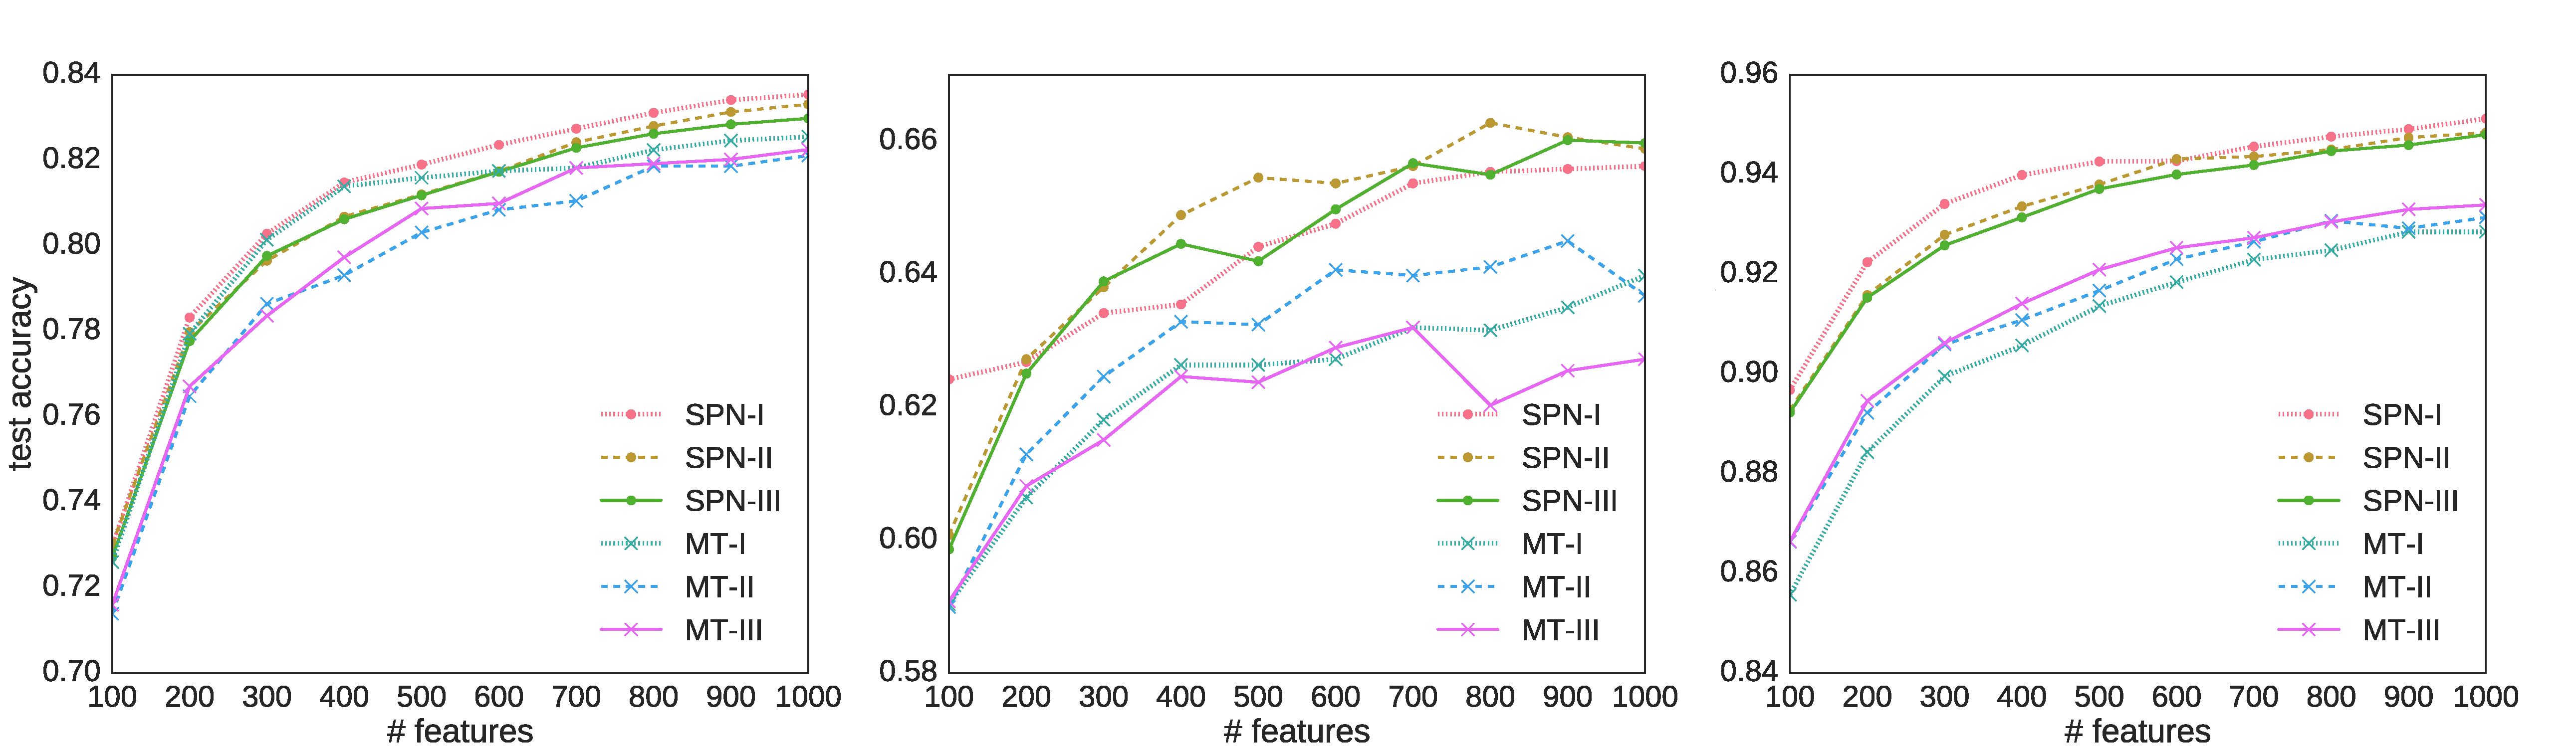
\includegraphics[width=1.0\linewidth]{figures/lines-wide}
  \end{center}
  \footfullcitenomarkleft{Vergari2016a}
  % Two general extraction schemes: random query construction and random
  % `patch' estimation
\end{frame}

\begin{frame}
  \frametitle{Encoding/Decoding Embeddings}
  MPN as autoencoders\footnote{Vergari et al. Encoding and Decoding
    Representations with Sum-Product Networks, 2016, to appear}.
\end{frame}




\section{Applications}
{\setbeamertemplate{headline}{}
  \begin{frame}[c]
    \sectionpage
  \end{frame}
}

\begin{frame}
  \frametitle{Applications I: computer vision}
  
\end{frame}


\begin{frame}
  \frametitle{Applications II: language modeling}
  
\end{frame}

\begin{frame}
  \frametitle{Applications III: activity recognition}
\end{frame}

\begin{frame}
  \frametitle{Applications IV: speech}
  SPNs to model the joint pdf of observed RVs in HMMs (HMM-SPNs).
  \begin{center}
    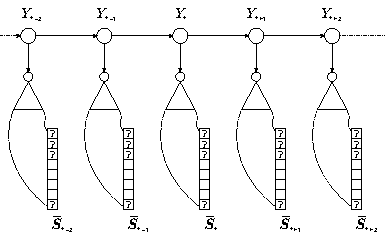
\includegraphics[width=0.35\columnwidth]{figures/peharz2014a-figures/hmm-spn-model}
  \end{center}\par\bigskip

  State-of-the-art high frequency reconstruction (MPE inference)
  \begin{center}
    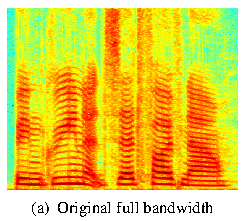
\includegraphics[width=0.25\columnwidth]{figures/peharz2014a-figures/orig}
    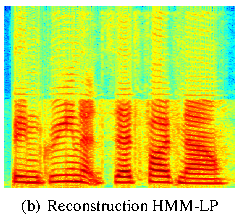
\includegraphics[width=0.25\columnwidth]{figures/peharz2014a-figures/hmm-lp}
    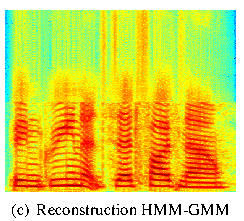
\includegraphics[width=0.25\columnwidth]{figures/peharz2014a-figures/hmm-gmm}
    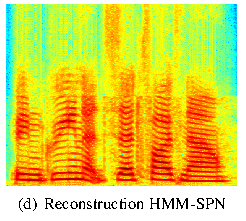
\includegraphics[width=0.25\columnwidth]{figures/peharz2014a-figures/hmm-spn}
  \end{center}
  
  \footfullcitenomarkleft{Peharz2014a}
\end{frame}


\begin{frame}
  \frametitle{Trends \& What to do next}
  Scalable structure learning
  Continuous RVs structure learning

  End-to-end training with hybrid NN architectures
\end{frame}

\section{References}
{\setbeamertemplate{headline}{}
  \begin{frame}[c]
    \sectionpage
  \end{frame}
}

\begin{frame}
  \frametitle{awesome-spn}
  A curated and structured list of resources about SPNs\footnote{Inspired by the
    SPN page {http://spn.cs.washington.edu/} at the Washington  University}.

  \url{https://github.com/arranger1044/awesome-spn}
\end{frame}

%\begin{frame} [allowframebreaks]
%  \setbeamertemplate{bibliography item}{}
%  \setlength\bibitemsep{8pt}
%  \printbibliography
%\end{frame}




\end{document}


%%% Local Variables:
%%% mode: latex
%%% TeX-master: t
%%% TeX-engine: xetex
%%% End:
